\chapter{La couche ISA}

%% Schéma général avec les différents composants : microprocesseur, mémoire, périphériques, bus de communication.

%% \todo{architecture de von Neumann}
%% \begin{figure}[htbp]
%% \centering toto
%% \caption{Architecture de von Neumann : }
%% \end{figure}

Nous avions terminé la section précédente en utilisant un chemin de données séquencé manuellement. Nous avons d'ailleurs introduit deux couches d'architecture (fig.\ref{fig:couches_architecture}): une couche physique et une couche logique. La couche physique concerne la réalisation électronique, en utilisant notamment des transistors, de portes logiques. La couche logique, qui contient tout les circuits de logique combinatoire et séquentielle, offre un premier niveau d'abstraction : lorsqu'on parle de logique, on ne mentionne plus les transistors et on pourrait tout à fait concevoir de réaliser la couche physique sous-jacente avec une autre technologique (e.g. optique) sans pour autant que les raisonnements au niveau de la couche logique ne soit affecté. Dans cette partie, on ajoute encore un niveau d'abstraction : la couche ISA ``\emph{Instruction Set Architecture}''. Ce niveau d'abstraction supplémentaire va nous permettre de nous détacher encore un plus de la réalisation matérielle/physique de la machine et nous faciliter aussi son utilisation.

\begin{figure}[htbp]
\centering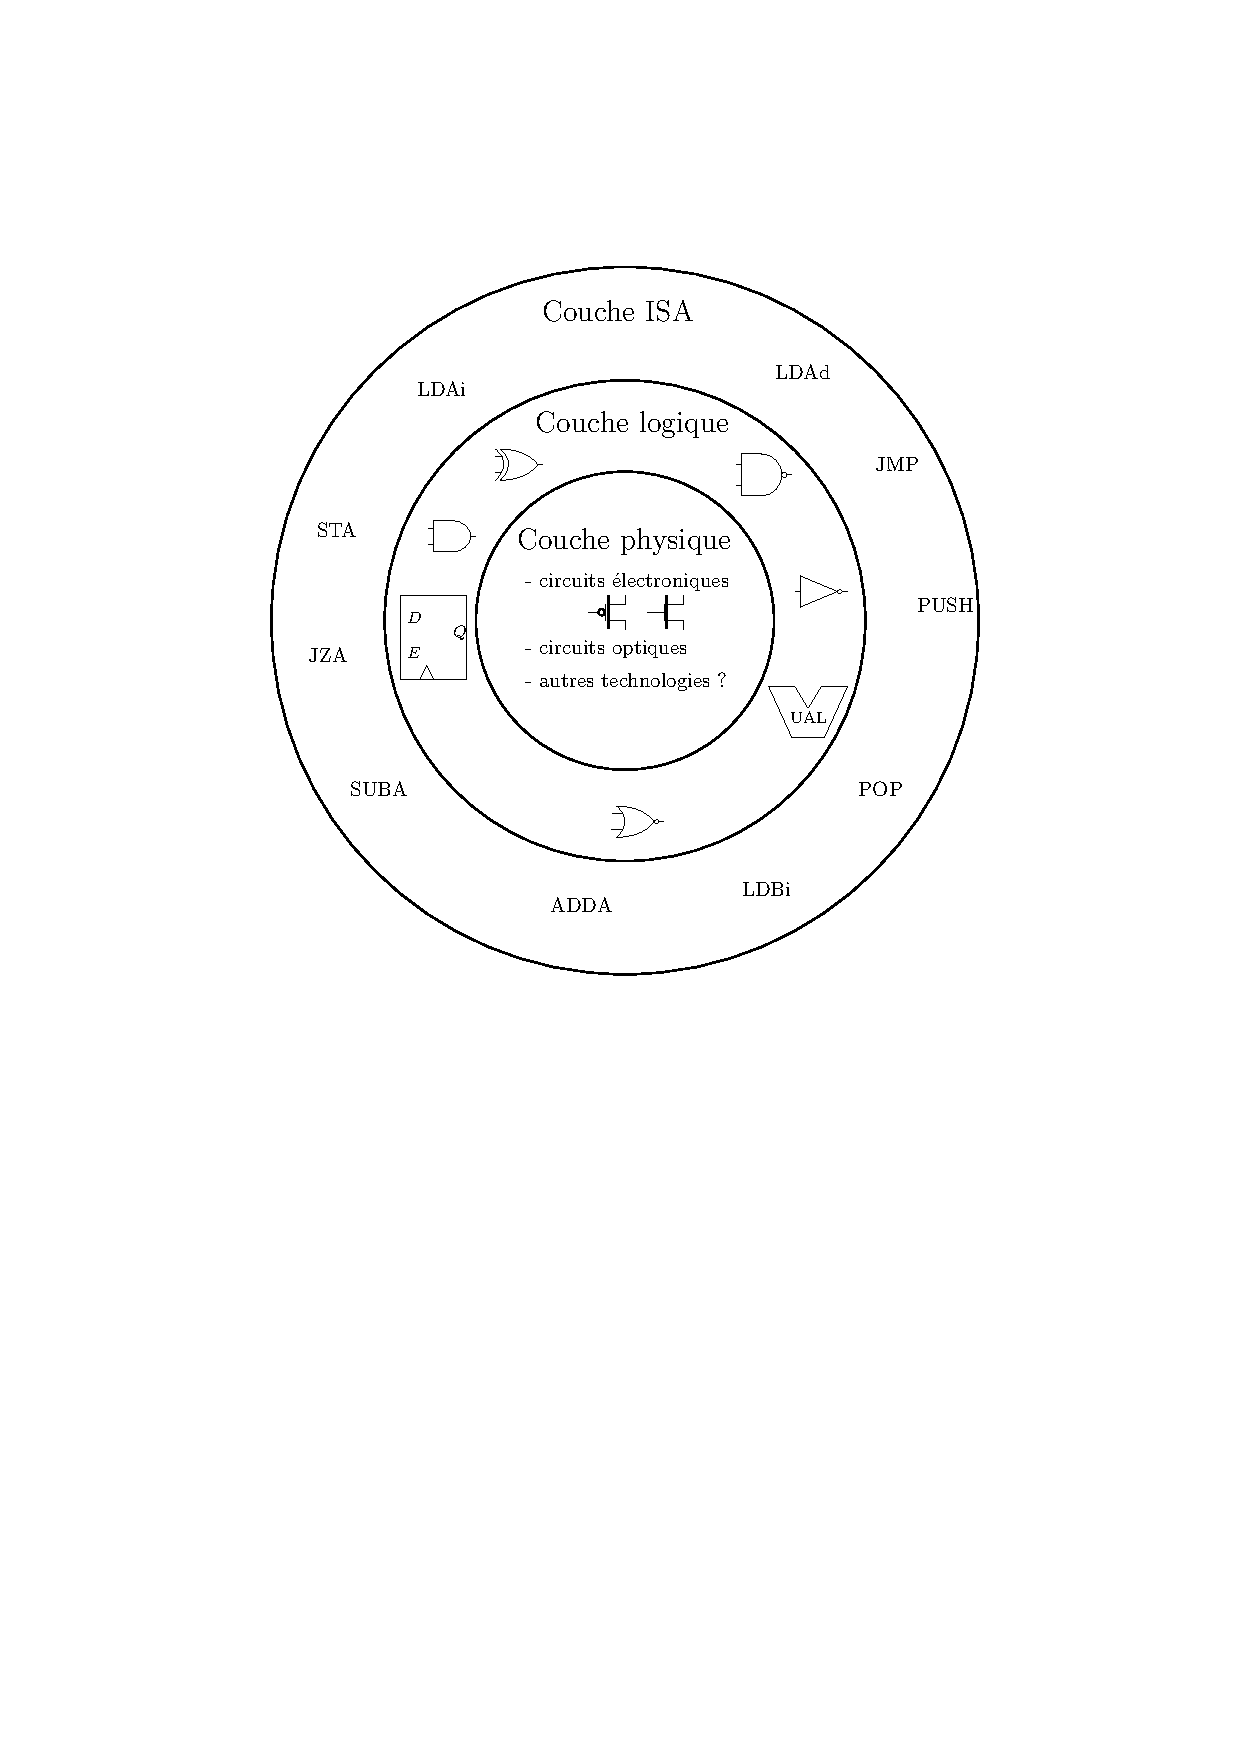
\includegraphics[width=0.6\linewidth]{Figs/couches_architecture.pdf}
\caption{\label{fig:couches_architecture} Dans cette partie on introduit une nouvelle couche d'abstraction : la couche ISA qui permet de se détacher un peu de la réalisation matérielle sous-jacente de la machine.}
\end{figure}

Ce qui rend l'utilisation de l'architecture plus facile en ajoutant des couches d'abstraction, c'est qu'à chaque fois qu'on traverse une couche d'abstraction, on change la nature des spécifications de l'architecture (fig.\ref{fig:couches_architecture_specif}). 

\begin{figure}[htbp]
\centering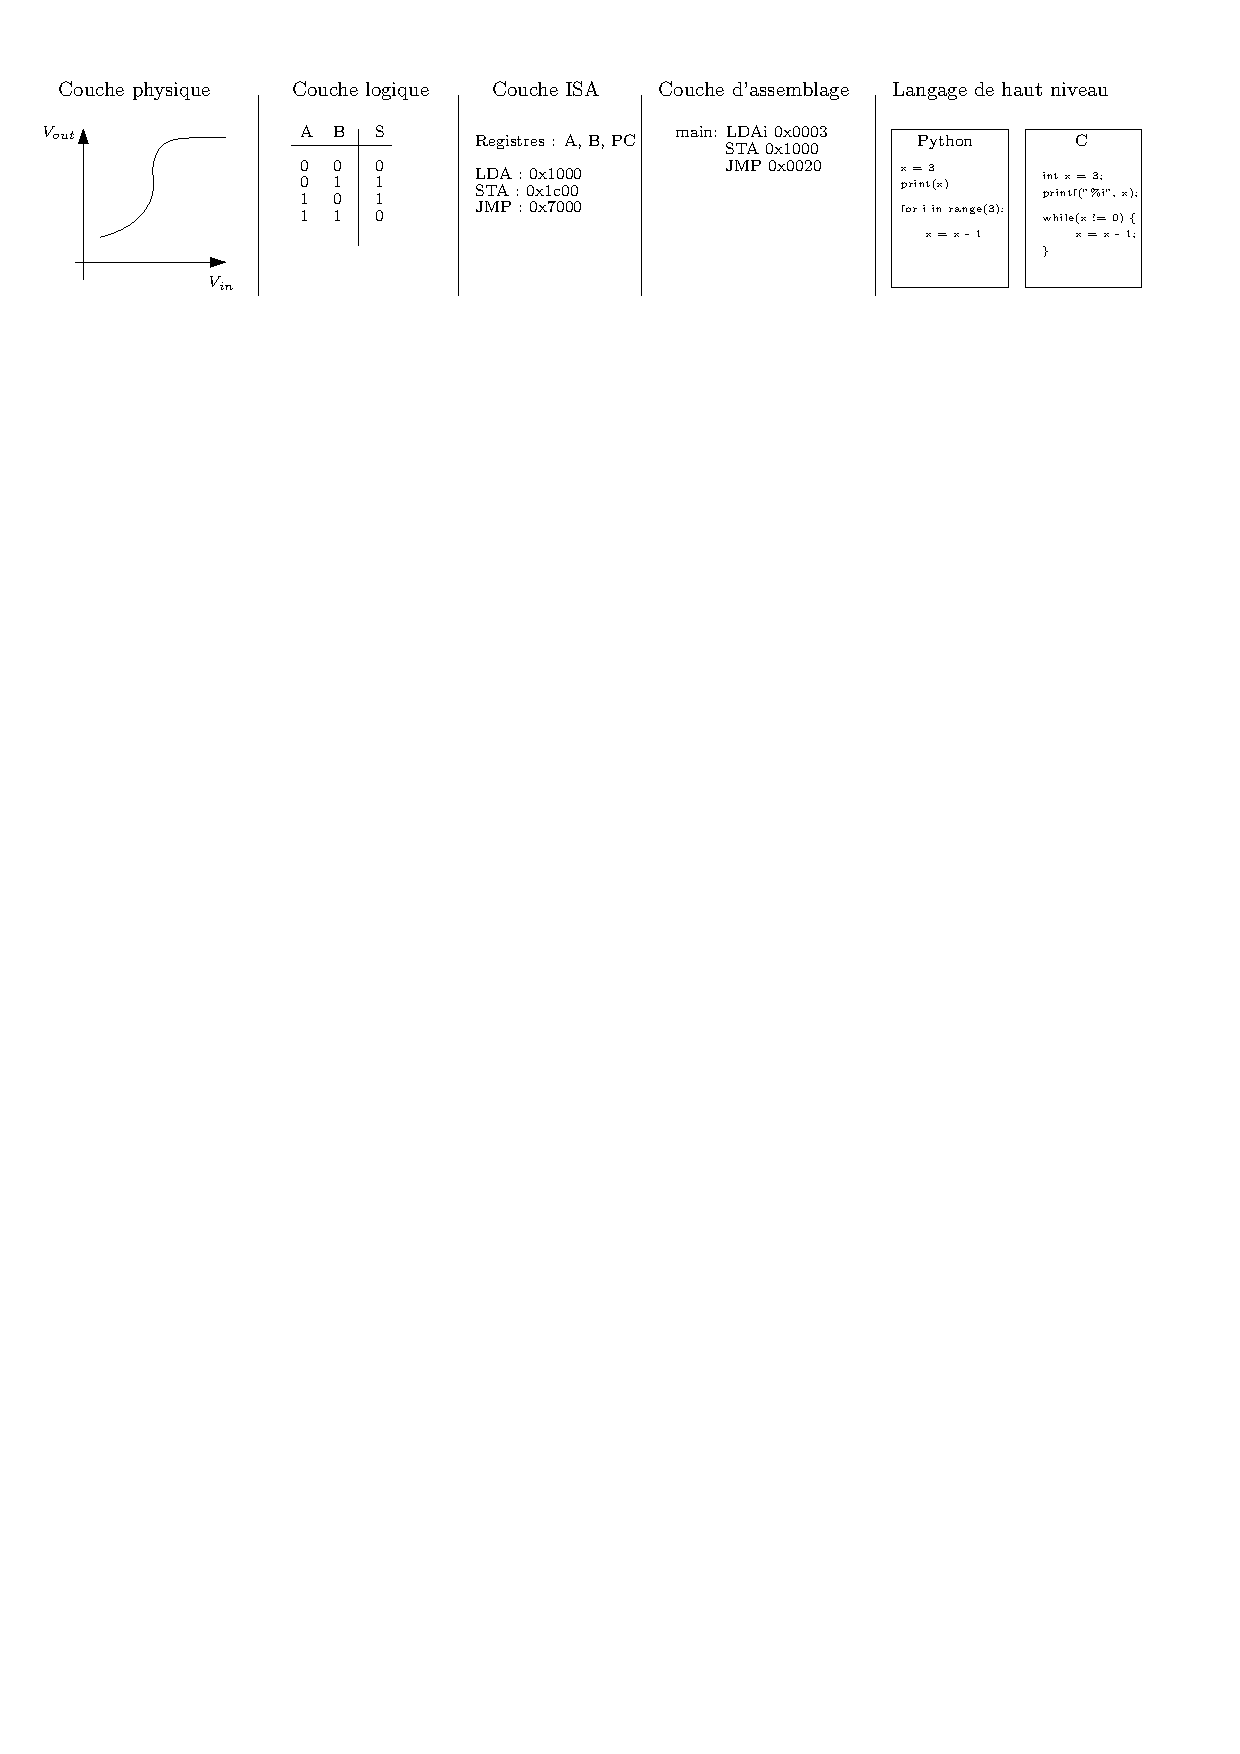
\includegraphics[width=\linewidth]{Figs/couches_architecture_specif.pdf}
\caption{\label{fig:couches_architecture_specif} Chaque fois qu'une nouvelle couche d'abstraction est introduite, les spécifications fonctionnelles de l'architecture change de nature et cela facilite son utilisation.}
\end{figure}

Par exemple, les spécifications fonctionnelles de la couche physique, lorsque nous avons introduit les transitors, sont données en terme de fonction de transfert caractéristique $V_{out} = f(V_{in})$ faisant intervenir les tensions d'entrée et de sortie. Les spécifications logiques sont données sous la forme de tables de vérité, et on raisonne alors en termes d'états binaires d'entrée et de sortie plutôt qu'en terme de tensions d'entrée et de sortie. La couche ISA spécifie des registres, des opérations réalisables et des instructions (nous allons voir ça dans un instant) pour manipuler leurs contenus : LOADA, STA, ADDA. Nous verrons dans le prochain chapitre une autre couche d'abstraction introduite par les langages de haut niveau, comme Python, C, C++, qui apporte une plus grande souplesse dans la programmation mais également une abstraction de l'architecture telle que ce sera exactement le même propgramme qui pourra être exécuté sur plusieurs architectures. Après cette petite parenthèse, concentrons nous sur la couche ISA \emph{Instruction Set Architecture} et voyons comment automatiser le séquencement du chemin de données. Pour cela, il faut résoudre deux problèmes:
\begin{itemize}
\item comment indiquer à la machine la séquence d'instructions à exécuter ?
\item étant donnée une instruction, comment générer la séquence de micro-instructions, i.e. la séquence de signaux de contrôle du chemin de données
\end{itemize}
Au même titre que nous avons établi un code binaire pour représenter des entiers, des caractères, etc... on va se donner un code binaire pour coder les instructions et on va placer ces instructions dans la RAM. C'est d'ailleurs un des principes de l'architecture de von Neumann que de placer indifféremment les instructions et les données en RAM. Au même titre que lorsqu'on voit le mot binaire $1000001$, on ne sait pas d'après le mot si la valeur est un A codé en ASCII, $-63$ codé en complément à deux ou l'entier naturel $65$, ce n'est pas le code qui vous dit qu'un mot est une instruction ou une donnée, mais c'est l'utilisation qu'on va en faire.

Le deuxième problème consiste à trouver un moyen de générer la séquence des signaux de contrôle qui permettent de réaliser les opérations que nous souhaitons réaliser avec le chemin de données. Générer une séquence de sorties se réalise très bien grâce à, ce qu'on appelle, un transducteur finis.

\section{Programme et données en mémoire}


% \subsection{Architecture de Von Neumann}

%\todo{Une introduction sur von Neumann}

\subsection{Codage des instructions en mémoire}

Reprenons l'exemple du chapitre précédent \ref{sec:chemin_donnes_exemple}. Le contenu de la RAM avec uniquement les opérandes est représenté à nouveau sur la figure \ref{fig:ram_data_prog_op}. 

\begin{figure}[htbp]
\centering\begin{tabular}{l|cccc}
Adresses & \multicolumn{4}{c}{Contenu}\\
\hline
0000 & 0010 & 0001 & 000A & 0000\\
0004 & 0000 & 0000 & 0000 & 0000\\
0008 & 0000 & 0000 & 0000 & 0000
\end{tabular}
\caption{\label{fig:ram_data_prog_op} Contenu de la RAM avec uniquement les opérandes tel que nous l'avons considéré dans la section \ref{sec:chemin_donnes_exemple}.}
\end{figure}


Je vous propose une étape intermédiaire (qui pour le moment ne fait aucun sens puisque j'écris des caractères au lieu de nombres binaires !) en ajoutant les instructions dans la RAM sur la figure \ref{fig:ram_data_prog}a. On indique alors directement en RAM le programme qui, ici, consiste~:
\begin{enumerate}
\item à charger dans le registre A la valeur $0\times0010$,
\item puis à charger dans le registre B la valeur $0\times0001$,
\item puis à additionner le contenu des registres A et B et stocker le résultat dans le registre A
\item et enfin à sauvegarder la valeur du registre A en RAM à l'adresse $0\times000A$.
\end{enumerate}

Donnons nous maintenant un code, qui pour le moment vous paraîtra totalement arbitraire mais qui le sera moins dans les sections qui suivent. En tout cas, donnons nous le code sur 16 bits comme dans la table~\ref{table:code_op1}.

\begin{table}[htbp]
\centering\begin{tabular}{c|c}
Nom de l'instruction & Code de l'instruction \\
\hline
LDAi & $0\times1000$\\
LDAd & $0\times1400$\\
LDBi & $0\times2000$\\
STA  & $0\times1c00$\\
ADDA & $0\times3000$
\end{tabular}
\caption{\label{table:code_op1} Codes binaires sur 16 bits des instructions LDAi, LDAd, LDBi, STA et ADDA considérées jusqu'à maintenant}
\end{table}

Armés de ces codes d'instruction, nous pouvons maintenant produire le contenu de la RAM en remplaçant les instructions par leur code telle que sur la figure~\ref{fig:ram_data_prog}b.

\begin{figure}[htbp]
\centering\begin{tabular}{cc}
\begin{tabular}{l|cccc}
Adresses & \multicolumn{4}{c}{Contenu}\\
\hline
0000 & \texttt{LDAi} & 0010 & \texttt{LDBi} & 0001\\
0004 & \texttt{ADDA} & \texttt{STA} & 000A & 0000\\
0008 & 0000 & 0000 & 0000 & 0000
\end{tabular}& 
\begin{tabular}{l|cccc}
Adresses & \multicolumn{4}{c}{Contenu}\\
\hline
0000 & 1000 & 0010 & 2000 & 0001\\
0004 & 3000 & 1c00 & 000A & 0000\\
0008 & 0000 & 0000 & 0000 & 0000
\end{tabular}\\
a) & b)
\end{tabular}
\caption{\label{fig:ram_data_prog} a) Contenu de la RAM dont nous aimerions disposer pour indiquer à la machine la séquence des instructions à appliquer. b) Contenu de la RAM une fois les instructions codées en binaire.}
\end{figure}

Nous venons d'écrire notre premier programme \textbf{en langage machine}. Tout est dans la RAM : le programme et les données. En voyant ce morceau de RAM et en connaissant les codes des instructions, vous êtes capable de comprendre ce que fait ce programme (ce qui n'était pas le cas avant puisque vous n'aviez que les opérandes et ne saviez donc pas quoi en faire !); Il suffit d'appliquer le raisonnement suivant :
\begin{itemize}
\item la RAM commence à l'adresse $0\times0000$ par une instruction
\item la première instruction a le code $0\times1000$ et donc c'est l'instruction LDAi
\item comme LDAi a besoin d'une seule opérande, le seul mot suivant est cette opérande
\item puis vient une autre instruction de code $0\times2000$ qui corresponds à l'instruction LDBi
\item comme LDBi a besoin d'une seule opérande, le seul mot suivant est cette opérande
\item puis vient une autre instruction de code $0\times3000$ qui corresponds à l'instruction ADDA qui n'a pas besoin d'opérande
\item puis vient une autre instruction de code $0\times1c00$ qui corresponds à l'instruction STA
\item comme STA a besoin d'une seule opérande, le seul mot suivant est cette opérande
\end{itemize}
 Voyons maintenant comment automatiser l'exécuter de ce programme. 

\subsection{Récupérer l'instruction depuis la mémoire (\emph{fetch})}

Le fait d'introduire les instructions dans la RAM nécessite de changer un peu la façon dont le séquenceur utilise la mémoire. En effet, on ne traite plus uniquement des opérandes mais il faut également extraire les instructions de la mémoire, ce qu'on appelle la \textbf{phase de fetch}. 

\begin{figure}
\includegraphics[width=\linewidth]{Figs/premier_chemin_ri.pdf}
\caption{\label{fig:premier_chemin_ri} Chemin de données avec le registre d'instruction (RI), un registre dédié à mémoriser l'instruction en cours d'exécution. Ce registre n'a besoin d'être accessible en lecture que par le séquenceur.}
\end{figure}

On ajoute au chemin de données un registre, le \textbf{registre d'instruction} (RI), un régistre dédié à la mémorisation de l'instruction en cours d'exécution. Le chemin de données est alors un peu modifié comme sur la figure~\ref{fig:premier_chemin_ri}. Pour rester homogène avec l'introduction des autres registres, le registre d'instruction est connecté sur le bus de sortie de l'UAL mais rien ne l'oblige puisque les instructions seront toujours fournies par la RAM. Aussi, la sortie du registre d'instruction est redirigée vers le séquenceur (ce qui est responsable d'orchestrer le chemin de données, i.e. vous pour le moment) qui est le seul élément qui a besoin de connaître l'instruction en cours d'exécution. 

Les micro-instructions pour la phase de fetch sont assez simples, elles consistent simplement à charger le contenu de la RAM dans le registre d'instruction et à incrémenter le PC : \texttt{RI:=RAM[PC] ; PC:=PC+1}.

\section{Générer les micro-instructions par une machine à états finis}

Lorsque nous avons introduit notre premier chemin de données à la fin du chapitre précédent, nous avons exécuté des instructions et chacune de ces instructions nécessitait une séquence de micro-instructions c'est à dire une séquence de signaux de contrôle. En informatique, produire une séquence de sorties (éventuellement dépendantes d'entrées) se représente bien sous la forme d'un automate à états finis\footnote{en toute rigueur, un transducteur finis. Un automate à états finis est constitué d'une collection d'états, dont des états initiaux et finaux, et de transitions éventuellement stochastiques entre les états. L'automate démarre dans un des états initiaux et les transitions sont empruntées en fonction des entrées reçues. Un transducteur fini rajoute des sorties générées soit en fonction des états, soit en fonction des transitions. Dans le cas de transitions déteministes, on parle de machine de Moore (lorsque les sorties ne dépendent que de l'état courant) et machine de Mealy (lorsque les sorties dépendent de l'état courant et des entrées)}.

\subsection{Une machine à états finis pour le fetch}

Commençons par voir comment générer la séquence de micro-instructions pour la phase de récupération de l'instruction, la phase de \textbf{fetch}. La phase de fetch consiste à~:
\begin{enumerate}
\item diriger le PC vers RADM, donc lire le PC (ReadPC=1), transférer l'entrée A vers la sortie S pour l'UAL (UAL=0000), stocker le résultat dans RADM (SetRADM=1) \textbf{et} déclencher un front montant d'horloge
\item diriger le contenu de la mémoire vers le registre RI, donc lire le contenu de la mémoire (ReadMem=1), transférer l'entrée B vers la sortie S de l'UAL (UAL=0001), stocker le résultat dans le registre RI (SetRI=1) \textbf{et} déclencher un front montant d'horloge
\item incrémenter le registre PC, donc lire le PC (ReadPC=1), incrémenter l'entrée A de l'UAL (UAL=1000), stocker le résultat dans le registre PC (SetPC=1) \textbf{et} déclencher un front montant d'horloge
\end{enumerate}

Cette séquence peut se représenter graphiquement sous la forme d'un transducteur finis comme sur la figure \ref{fig:transducteur_fetch}.

\begin{figure}[htbp]
  \centering\begin{tikzpicture}
    GraphInit[vstyle=Normal]
    \SetGraphUnit{3}
    \tikzset{LabelStyle/.style= {draw,
        fill  = yellow,
        text  = red},
      EdgeStyle/.style = {->}}
    \Vertex[Math,L=0,x=0,y=2]{A}
    \Vertex[Math,L=1,x=4,y=2]{B}
    \Vertex[Math,L=2,x=8,y=2]{C}
    \Vertex[Math,L=3,x=10,y=2]{D}
    \Edge(A)(B)
    \Edge(B)(C)
    \Edge(C)(D)
    \node[text width=2cm] at ($(A) - (0,1)$) {ReadPC=1\\UAL=0000\\SetRADM=1} ;
    \node[text width=2cm] at ($(B) - (0,1)$) {ReadMem=1\\UAL=0001\\SetRI=1} ;
    \node[text width=2cm] at ($(C) - (0,1)$) {ReadPC=1\\UAL=1000\\SetPC=1} ;
  \end{tikzpicture}
  \caption{\label{fig:transducteur_fetch} Machine à états générant les micro-instructions pour récupérer l'instruction \texttt{RI := MEM[PC]; PC:=PC+1}. Les transitions sont empruntées à chaque front montant d'horloge.}
\end{figure}

Pour exécuter l'instruction de fetch, il suffit alors de démarrer l'automate dans l'état 0 et d'emprunter les transitions à chaque front montant d'horloge.

\subsection{Une machine à états finis par instruction}

Pour définir les machines à états pour les instructions, reprenons l'exemple du chargement immédiat d'une opérande de la RAM vers le registre A. Nous noterons cette instruction \textbf{LDAi}. La séquence de micro-instructions que nous avons considérées est la suivante :
\begin{enumerate}
\item diriger le PC vers RADM, donc lire le PC (ReadPC=1), transférer l'entrée A vers la sortie S pour l'UAL (UAL=0000), stocker le résultat dans RADM (SetRADM=1) \textbf{et} déclencher un front montant d'horloge
\item diriger le contenu de la mémoire vers le registre A, donc lire le contenu de la mémoire (ReadMem=1), transférer l'entrée B vers la sortie S de l'UAL (UAL=0001), stocker le résultat dans le registre A (SetA=1) \textbf{et} déclencher un front montant d'horloge
\item incrémenter le registre PC, donc lire le PC (ReadPC=1), incrémenter l'entrée A de l'UAL (UAL=1000), stocker le résultat dans le registre PC (SetPC=1) \textbf{et} déclencher un front montant d'horloge
\end{enumerate}

Cette séquence peut se représenter graphiquement sous la forme d'un transducteur finis comme sur la figure \ref{fig:transducteur_ldai}.

\begin{figure}[htbp]
  \centering\begin{tikzpicture}
    GraphInit[vstyle=Normal]
    \SetGraphUnit{3}
    \tikzset{LabelStyle/.style= {draw,
        fill  = yellow,
        text  = red},
      EdgeStyle/.style = {->}}
    \Vertex[Math,L=0,x=0,y=2]{A}
    \Vertex[Math,L=1,x=4,y=2]{B}
    \Vertex[Math,L=2,x=8,y=2]{C}
    \Vertex[Math,L=3,x=10,y=2]{D}
    \Edge(A)(B)
    \Edge(B)(C)
    \Edge(C)(D)
    \tikzset{VertexStyle/.append style={rectangle}}
    \node[text width=2cm] at ($(A) - (0,1)$) {ReadPC=1\\UAL=0000\\SetRADM=1} ;
    \node[text width=2cm] at ($(B) - (0,1)$) {ReadMem=1\\UAL=0001\\SetA=1} ;
    \node[text width=2cm] at ($(C) - (0,1)$) {ReadPC=1\\UAL=1000\\SetPC=1} ;
  \end{tikzpicture}
  \caption{\label{fig:transducteur_ldai} Machine à états générant les micro-instructions pour le chargement immédiat d'une opérande dans le registre A. Les transitions sont empruntées à chaque front montant d'horloge. L'instruction sera notée \textbf{LDAi}.}
\end{figure}

Les états sont numérotés $0$, $1$, $2$ et $3$, $0$ étant l'état initial et $3$ l'état final. Sous chacun des états se trouve l'état des signaux de contrôle. Les signaux de contrôle qui ne sont pas précisés sont à $0$. Les transitions sont empruntées à chaque front montant d'horloge et sont ici indépendantes des entrées (ce qui ne sera pas le cas pour quelques instructions comme les branchements). On peut de la même façon construire des machines à états pour les autres instructions mentionnées dans la section \ref{sec:chemin_donnes_exemple}. Pour l'instruction de chargement immédiat dans le registre B, que nous noterons \textbf{LDBi}, la machine à état est donnée sur la figure \ref{fig:transducteur_ldbi}.

\begin{figure}[htbp]
  \centering\begin{tikzpicture}
    GraphInit[vstyle=Normal]
    \SetGraphUnit{3}
    \tikzset{LabelStyle/.style= {draw,
        fill  = yellow,
        text  = red},
      EdgeStyle/.style = {->}}
    \Vertex[Math,L=0,x=0,y=2]{A}
    \Vertex[Math,L=1,x=4,y=2]{B}
    \Vertex[Math,L=2,x=8,y=2]{C}
    \Vertex[Math,L=3,x=10,y=2]{D}
    \Edge(A)(B)
    \Edge(B)(C)
    \Edge(C)(D)
    \node[text width=2cm] at ($(A) - (0,1)$) {ReadPC=1\\UAL=0000\\SetRADM=1} ;
    \node[text width=2cm] at ($(B) - (0,1)$) {ReadMem=1\\UAL=0001\\SetB=1} ;
    \node[text width=2cm] at ($(C) - (0,1)$) {ReadPC=1\\UAL=1000\\SetPC=1} ;
  \end{tikzpicture}
  \caption{\label{fig:transducteur_ldbi} Machine à états générant les micro-instructions pour le chargement immédiat d'une opérande dans le registre B. Les transitions sont empruntées à chaque front montant d'horloge. L'instruction sera notée \textbf{LDBi}.}
\end{figure}

Pour l'instruction additionnant le contenu des registres A et B et stockant le résultat dans le registre A, que nous noterons \textbf{ADDA}, la machine à état est donnée sur la figure \ref{fig:transducteur_adda}.

\begin{figure}[htbp]
  \centering\begin{tikzpicture}
    GraphInit[vstyle=Normal]
    \SetGraphUnit{3}
    \tikzset{LabelStyle/.style= {draw,
        fill  = yellow,
        text  = red},
      EdgeStyle/.style = {->}}
    \Vertex[Math,L=0,x=0,y=2]{A}
    \Vertex[Math,L=1,x=4,y=2]{B}
    \Edge(A)(B)
    \node[text width=2cm] at ($(A) - (0,1)$) {ReadA=1\\ReadB=1\\UAL=0110\\SetA=1} ;
  \end{tikzpicture}
  \caption{\label{fig:transducteur_adda} Machine à états générant les micro-instructions pour l'addition du contenu des registres A et B, le résultant étant sauvegardé dans le registre A. Les transitions sont empruntées à chaque front montant d'horloge. L'instruction sera notée \textbf{ADDA}. Il n'y a pas à incrémenter le PC puisqu'aucune opérande n'est consommée en RAM.}
\end{figure}

Pour l'instruction stockant le contenu du registre A en mémoire à l'adresse stockée en RAM à l'adresse stockée dans PC, que nous noterons \textbf{STA}, la machine à état est donnée sur la figure \ref{fig:transducteur_sta}.

\begin{figure}[htbp]
  \centering\begin{tikzpicture}
    GraphInit[vstyle=Normal]
    \SetGraphUnit{3}
    \tikzset{LabelStyle/.style= {draw,
        fill  = yellow,
        text  = red},
      EdgeStyle/.style = {->}}
    \Vertex[Math,L=0,x=0,y=2]{A}
    \Vertex[Math,L=1,x=3,y=2]{B}
    \Vertex[Math,L=2,x=6,y=2]{C}
    \Vertex[Math,L=3,x=9,y=2]{D}
    \Vertex[Math,L=4,x=12,y=2]{E}
    \Edge(A)(B)
    \Edge(B)(C)
    \Edge(C)(D)
    \Edge(D)(E)
    \tikzset{VertexStyle/.append style={rectangle}}
    \node[text width=2cm] at ($(A) - (0,1)$) {ReadPC=1\\UAL=0000\\SetRADM=1} ;
    \node[text width=2cm] at ($(B) - (0,1)$) {ReadMem=1\\UAL=0001\\SetRADM=1} ;
    \node[text width=2cm] at ($(C) - (0,1)$) {ReadA=1\\UAL=0000\\SetMem=1} ;
    \node[text width=2cm] at ($(D) - (0,1)$) {ReadPC=1\\UAL=1000\\SetPC=1} ;
  \end{tikzpicture}
  \caption{\label{fig:transducteur_sta} Machine à états générant les micro-instructions pour la sauvegarde du contenu du registre A à l'adresse \texttt{RAM[PC]}. Les transitions sont empruntées à chaque front montant d'horloge. L'instruction sera notée \textbf{STA}.}
\end{figure}

Il nous reste une dernière instruction que nous avons évoqué lors de l'exemple de la section \ref{sec:chemin_donnes_exemple} : le chargement direct. Pour l'instruction chargeant dans le registre A le contenu de la mémoire \texttt{RAM[RAM[PC]]}, que nous noterons \textbf{LDAd}, la machine à état est donnée sur la figure \ref{fig:transducteur_ldad}.

\begin{figure}[htbp]
  \centering\begin{tikzpicture}
    GraphInit[vstyle=Normal]
    \SetGraphUnit{3}
    \tikzset{LabelStyle/.style= {draw,
        fill  = yellow,
        text  = red},
      EdgeStyle/.style = {->}}
    \Vertex[Math,L=0,x=0,y=2]{A}
    \Vertex[Math,L=1,x=3,y=2]{B}
    \Vertex[Math,L=2,x=6,y=2]{C}
    \Vertex[Math,L=3,x=9,y=2]{D}
    \Vertex[Math,L=4,x=12,y=2]{E}
    \Edge(A)(B)
    \Edge(B)(C)
    \Edge(C)(D)
    \Edge(D)(E)
    \node[text width=2cm] at ($(A) - (0,1)$) {ReadPC=1\\UAL=0000\\SetRADM=1} ;
    \node[text width=2cm] at ($(B) - (0,1)$) {ReadMem=1\\UAL=0001\\SetRADM=1} ;
    \node[text width=2cm] at ($(C) - (0,1)$) {ReadMem=1\\UAL=0001\\SetA=1} ;
    \node[text width=2cm] at ($(D) - (0,1)$) {ReadPC=1\\UAL=1000\\SetPC=1} ;
  \end{tikzpicture}
  \caption{\label{fig:transducteur_ldad} Machine à états générant les micro-instructions pour le chargement direct d'une opérande dans le registre A : \texttt{A := RAM[RAM[PC]];PC:=PC+1}. Les transitions sont empruntées à chaque front montant d'horloge. L'instruction sera notée \textbf{LDAd}.}
\end{figure}

\subsection{Une machine à états finis pour toutes les instructions}

Nous venons de voir différentes machines à états finis permettant de générer les séquences de micro-instruction pour la phase de fetch (fig~\ref{fig:transducteur_fetch}) ainsi que pour les instructions LDAi (fig~\ref{fig:transducteur_ldai}), LDAd (fig~\ref{fig:transducteur_ldad}), LDBi (fig~\ref{fig:transducteur_ldbi}), STA (fig~\ref{fig:transducteur_sta}) et ADDA (fig~\ref{fig:transducteur_adda}). On peut agréger toutes ces machines à état pour en construire une plus grande qui soit capable de générer les micro-instructions pour 1) récupérer l'instruction à exécuter et 2) exécuter cette instruction. Cette machine à état peut ressembler à celle de la figure \ref{fig:transducteur_seq}.

\begin{figure}[htbp]
  \centering\begin{tikzpicture}[thick,scale=0.7, every node/.style={scale=0.7}]
    GraphInit[vstyle=Normal]
    \SetGraphUnit{3}
    \tikzset{LabelStyle/.style= {draw,
        fill  = white,
        text  = blue},
      EdgeStyle/.style = {->}}
    \Vertex[Math,L=Fetch0,x=-11,y=8]{A0}
    \Vertex[Math,L=Fetch1,x=-8,y=8]{B0}
    \Vertex[Math,L=Fetch2,x=-5,y=8]{C0}
    \Edge(A0)(B0)
    \Edge(B0)(C0)
    \node[text width=2cm] at ($(A0) - (0,1.5)$) {ReadPC=1\\UAL=0000\\SetRADM=1} ;
    \node[text width=2cm] at ($(B0) - (0,1.5)$) {ReadMem=1\\UAL=0001\\SetRI=1} ;
    \node[text width=2cm] at ($(C0) - (0,1.5)$) {ReadPC=1\\UAL=1000\\SetPC=1} ;


    \Vertex[Math,L=LDAi0,x=0,y=14]{A1}
    \Vertex[Math,L=LDAi1,x=4,y=14]{B1}
    \Vertex[Math,L=LDAi2,x=8,y=14]{C1}
    \Vertex[Math,L=Fetch0,x=10,y=14]{D1}
    \Edge(A1)(B1)
    \Edge(B1)(C1)
    \Edge(C1)(D1)
    \node[text width=2cm] at ($(A1) - (0,1.5)$) {ReadPC=1\\UAL=0000\\SetRADM=1} ;
    \node[text width=2cm] at ($(B1) - (0,1.5)$) {ReadMem=1\\UAL=0001\\SetA=1} ;
    \node[text width=2cm] at ($(C1) - (0,1.5)$) {ReadPC=1\\UAL=1000\\SetPC=1} ;

    \Vertex[Math,L=LDBi0,x=0,y=11]{A2}
    \Vertex[Math,L=LDBi1,x=4,y=11]{B2}
    \Vertex[Math,L=LDBi2,x=8,y=11]{C2}
    \Vertex[Math,L=Fetch0,x=10,y=11]{D2}
    \Edge(A2)(B2)
    \Edge(B2)(C2)
    \Edge(C2)(D2)
    \node[text width=2cm] at ($(A2) - (0,1.5)$) {ReadPC=1\\UAL=0000\\SetRADM=1} ;
    \node[text width=2cm] at ($(B2) - (0,1.5)$) {ReadMem=1\\UAL=0001\\SetB=1} ;
    \node[text width=2cm] at ($(C2) - (0,1.5)$) {ReadPC=1\\UAL=1000\\SetPC=1} ;


    \Vertex[Math,L=STA0,x=0,y=8]{A3}
    \Vertex[Math,L=STA1,x=2,y=8]{B3}
    \Vertex[Math,L=STA2,x=4,y=8]{C3}
    \Vertex[Math,L=STA3,x=8,y=8]{D3}
    \Vertex[Math,L=Fetch0,x=10,y=8]{E3}
    \Edge(A3)(B3)
    \Edge(B3)(C3)
    \Edge(C3)(D3)
    \Edge(D3)(E3)
    \node[text width=2cm] at ($(A3) - (0,1.5)$) {ReadPC=1\\UAL=0000\\SetRADM=1} ;
    \node[text width=2cm] at ($(B3) - (0,1.5)$) {ReadMem=1\\UAL=0001\\SetRADM=1} ;
    \node[text width=2cm] at ($(C3) - (0,1.5)$) {ReadA=1\\UAL=0000\\SetMem=1} ;
    \node[text width=2cm] at ($(D3) - (0,1.5)$) {ReadPC=1\\UAL=1000\\SetPC=1} ;




    \Vertex[Math,L=ADDA0,x=4,y=5]{A4}
    \Vertex[Math,L=Fetch0,x=10,y=5]{B4}
    \Edge(A4)(B4)
    \node[text width=2cm] at ($(A4) - (0,1.5)$) {ReadA=1\\ReadB=1\\UAL=0110\\SetA=1} ;

    \Vertex[Math,L=LDAd0,x=0,y=2]{A5}
    \Vertex[Math,L=LDAd1,x=2,y=2]{B5}
    \Vertex[Math,L=LDAd2,x=4,y=2]{C5}
    \Vertex[Math,L=LDAd3,x=8,y=2]{D5}
    \Vertex[Math,L=Fetch0,x=10,y=2]{E5}
    \Edge(A5)(B5)
    \Edge(B5)(C5)
    \Edge(C5)(D5)
    \Edge(D5)(E5)
    \node[text width=2cm] at ($(A5) - (0,1.5)$) {ReadPC=1\\UAL=0000\\SetRADM=1} ;
    \node[text width=2cm] at ($(B5) - (0,1.5)$) {ReadMem=1\\UAL=0001\\SetRADM=1} ;
    \node[text width=2cm] at ($(C5) - (0,1.5)$) {ReadMem=1\\UAL=0001\\SetA=1} ;
    \node[text width=2cm] at ($(D5) - (0,1.5)$) {ReadPC=1\\UAL=1000\\SetPC=1} ;


    \path[->]          (C0)  edge   [bend left=20]   node [fill=white,text=blue] {RI=$0\times1000$?} (A1);
    \path[->]          (C0)  edge   [bend left=20]   node [fill=white,text=blue] {RI=$0\times2000$?} (A2);
    \path[->]          (C0)  edge   []   node [fill=white,text=blue] {RI=$0\times1c00$?} (A3);
    \path[->]          (C0)  edge   [bend right=30]   node [fill=white,text=blue] {RI=$0\times3000$?} (A4);
    \path[->]          (C0)  edge   [bend right=20]   node [fill=white,text=blue] {RI=$0\times1400$?} (A5);
    %\Edge[label={toto}](C0)(A1)
    %\Edge[style={->,bend left},label={RI=$0 1000$?}](C0)(A1)
    %\Edge[style={->,bend left},label={RI=$0\times2000$?}](C0)(A2)
    %\Edge[style={->,bend right},label={RI=$0\times1c00$?}](C0)(A3)
    %\Edge[style={->,bend right},label={RI=$0\times3000$?}](C0)(A4)
    %\Edge[style={->,bend right},label={RI=$0\times1400$?}](C0)(A5)
  \end{tikzpicture}
  \caption{\label{fig:transducteur_seq} Machine à états générant les micro-instructions pour 1) transférer l'instruction à exécuter dans le registre RI et 2) exécuter l'instruction récupérée en ne considérant ici que les instructions LDAi, LDAd, LDBi, STA, ADDA et construite en agrégeant les machines à états \ref{fig:transducteur_fetch}, \ref{fig:transducteur_ldai},\ref{fig:transducteur_ldbi},\ref{fig:transducteur_sta},\ref{fig:transducteur_ldad}, \ref{fig:transducteur_adda}. Les transitions sont empruntées à chaque front montant d'horloge. L'état $Fetch0$ est l'état initial. A la fin de chaque instruction, on retourne à la phase de Fetch.}
\end{figure}

Avant d'exécuter une instruction, il faut la récupérer et la transférer dans le registre RI, donc la phase de fetch est commune à toutes les instructions et sa machine à états prefixe toutes les autres. En fonction de l'instruction récupérée pendant la phase de fetch, c'est l'une ou l'autre des machines à états qui est utilisée. Il nous faut maintenant voir comment réaliser cette machine à état et l'interfacer avec le chemin de données.


\section{Séquencement microprogrammé du chemin de données}

\subsection{Circuit logique du séquenceur microprogrammé et interface avec le chemin de données}

Nous avons présenté sur la figure \ref{fig:transducteur_seq} la machine à état permettant de générer les micro-instructions pour les instructions LDAi, LDBi, STA, LDAd. On s'intéresse maintenant au circuit logique réalisant cette machine à état. La réalisation de ce circuit logique est en fait, dans le principe, tout à fait similaire à l'illustration \ref{fig:intro_seq} lorsque nous avons introduit la logique séquentielle. Il nous faut un circuit calculant l'état suivant à partir de l'état courant et un circuit générant les sorties de contrôle à partir de l'état courant. Les signaux de contrôle, i.e. les microinstructions vont être mémorisées dans une ROM adressable par un registre et le contenu du registre contient l'état courant de la machine à état, comme illustré sur la figure~\ref{fig:sequenceur_micro}. Nous utilisons ici un registre MicroPC de $8$ bits, donc également une ROM adressable sur 8 bits (8 bits nous suffiront pour coder toutes les micro-instructions nécessaires pour l'architecture considérée dans ce cours). Jusqu'à maintenant, seuls 16 signaux de contrôle apparaissent sur le chemin de données mais, nous anticipons les évolutions à venir dans les prochains chapitres en utilisant une ROM contenant des mots de 32 bits.

\begin{figure}[htbp]
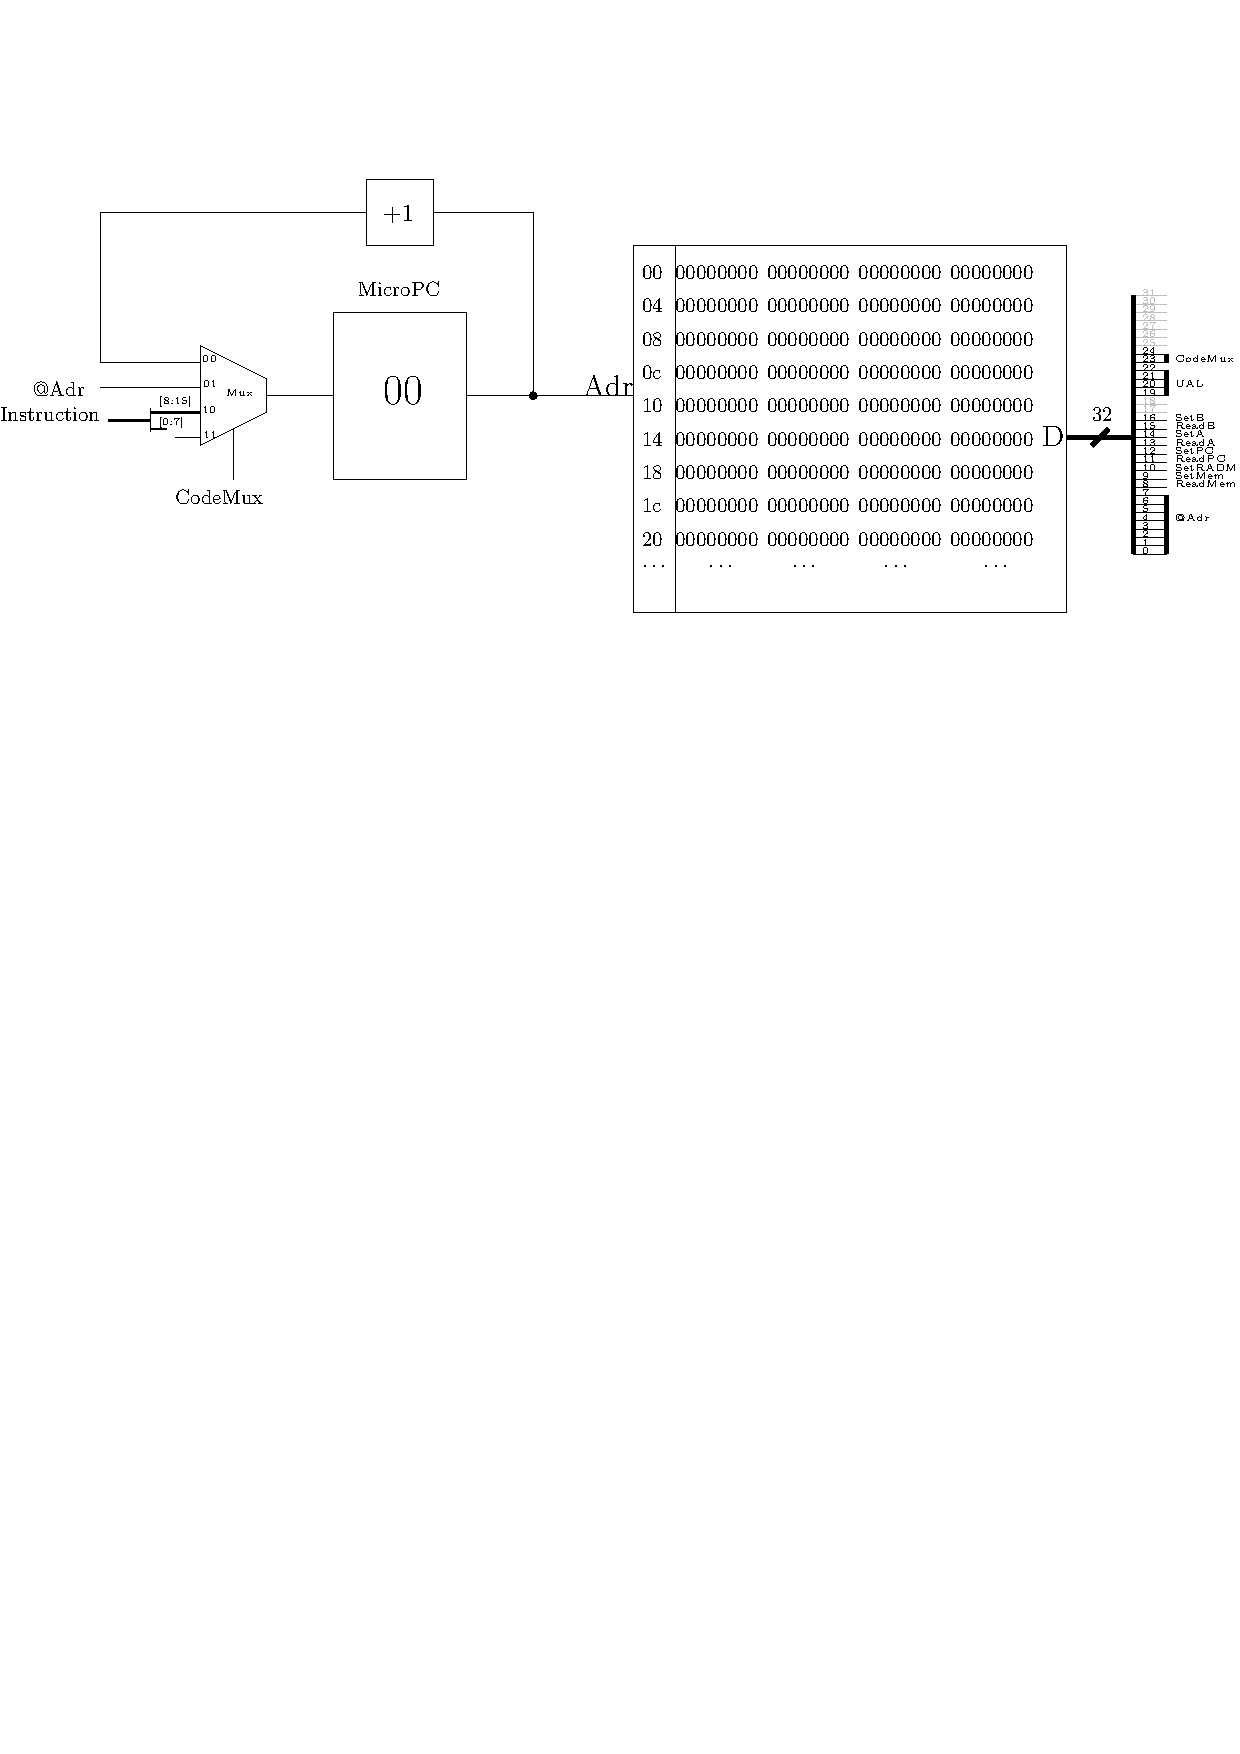
\includegraphics[width=\linewidth]{Figs/sequenceur_micro.pdf}
\caption{\label{fig:sequenceur_micro} Une première version du circuit logique d'un séquenceur micro-programmé. L'état est stocké dans le registre MicroPC qui adresse une ROM dont la sortie corresponds aux signaux de contrôle du chemin de données. La ROM est adressable sur 8 bits et contient des mots de 32 bits. Parmi les sorties de la ROM, celles qui ne sont pour le moment pas connectées au chemin de données sont grisées.}
\end{figure}

En pratique, les instructions que nous allons considérer dans notre réalisation ne nécessiteront jamais plus de 4 étapes de micro-instructions. Nous allons donc réserver 4 mots mémoire pour chaque instruction de notre architecture ainsi que 4 mots mémoires pour la phase de fetch/decode. L'instruction courante à exécuter, stockée dans le registre d'instruction, est codée sur 16 bits. Sur le schéma \ref{fig:sequenceur_micro}, seules les 8 bits de poids forts alimentent le multiplexeur en entrée du registre MicroPC. En ROM, on stockera les micro-instructions pour chaque instruction. A quelle adresse allons nous trouver ces micro-instructions ? et bien aux adresses qui sont les 8 bits de poids forts de nos codes d'instruction, à savoir : 
\begin{itemize}
\item entre les adresses 0x08 et 0x0b : micro-instructions pour la phase de fetch/decode,
\item entre les adresses 0x10 et 0x13 : micro-instructions de l'instruction \textbf{LDAi} (le code pour LDAi étant $0\times1000$,
\item entre les adresses 0x14 et 0x17 : micro-instructions de l'instruction \textbf{LDAd} (le code pour LDAi étant $0\times1400$,
\item entre les adresses 0x1c et 0x1f : micro-instructions de l'instruction \textbf{STA} (le code pour LDAi étant $0\times1c00$,
\item entre les adresses 0x20 et 0x23 : micro-instructions de l'instruction \textbf{LDBi} (le code pour LDAi étant $0\times2000$,
\item entre les adresses 0x30 et 0x33 : micro-instructions de l'instruction \textbf{ADDA} (le code pour LDAi étant $0\times3000$.
\end{itemize}
Le multiplexeur à l'entrée du registre MicroPC a un rôle particulier : c'est ce multiplexeur qui va, soit charger l'adresse de départ des micro-instructions si CodeMux=10, soit passer à l'adresse MicroPC+1 si CodeMux=00, soit charger une adresse fournie par les signaux de contrôle si CodeMux=01. C'est grâce à ce multiplexeur qu'on va pouvoir réaliser les branchements de la machine à états aux états Fetch2 et pour reboucler à l'état Fetch0. A chaque étape, il faudra configurer les bits de sélection du multiplexeur CodeMux pour :
\begin{itemize}
\item soit incrémenter le MicroPC en utilisant CodeMux=00
\item soit charger dans le MicroPC la valeur de l'entrée @Adr, en utilisant CodeMux=01
\item soit charger dans le MicroPC les 8 bits de poids fort de l'instruction, en utilisant CodeMux=10
\end{itemize}

L'interface entre le séquenceur micro-programmé et le chemin de données se fait de la manière suivante (fig.\ref{fig:premier_chemin_seq}) :
\begin{itemize}
\item le séquenceur a besoin de recevoir en entrée l'instruction a exécuter, on avait introduit le registre d'instruction dans le chemin de données et une première façon de faire est donc de connecter la sortie du registre d'instruction à l'entrée ``Instruction'' du séquenceur. Mais, il s'avère que dans le cas d'un séquenceur micro-programmé, le registre d'instruction est inutile et le séquenceur peut directement recevoir son entrée du bus B,
\item le séquenceur contrôle en sortie le chemin de données en produisant les micro-instructions. Nous utilisons ici 32 bits de sortie en prévision des évolutions qui vont venir dans les chapitres suivants. Les signaux de contrôle qui ne sont pour le moment pas utilisés sont grisés sur les figures du séquenceur.
\end{itemize}

\begin{figure}[htbp]
\includegraphics[width=\linewidth]{Figs/premier_chemin_seq.pdf}
\caption{\label{fig:premier_chemin_seq} Une première version de l'architecture comprenant le chemin de données, le séquenceur micro-programmé et la RAM.}
\end{figure}

Voyons maintenant comment remplir la ROM du séquenceur en reprenant toutes les micro-instructions de la phase fetch/decode et des instructions LDAi ($0\times1000$), LDAd($0\times1400$), LDBi($0\times2000$), STA($0\times1c00$) et ADDA($0\times3000$).

\paragraph{Initialisation :} le contenu du MicroPC étant $0\times00$, et comme nous devons commencer par la phase de fetch/decode, il faut charger dans le MicroPC l'adresse $0\times 08$. Il faut donc produire les signaux de contrôle CodeMux=$0b01$, @Adr=$0b000010000$, tous les autres signaux étant à 0, soit le mot binaire sur 32 bits, en séparant les paquets de 4 bits par des ``.'' pour plus de lisibilité, $0000.0000.1000.0000.0000.0000.0000.1000$, soit en hexadécimal $0\times00800008$.

\paragraph{Fetch/Decode :} n'ayant plus de registre d'instruction (parce qu'il ne va pas nous servir), il faut adapter un peu les signaux de contrôle que nous avions donnés lorsque nous avons définis la machine à états pour le fetch/decode. Il faut maintenant :
\begin{enumerate}
\item charger le PC dans RADM et incrémenter MicroPC, soit ReadPC=1, UAL=0000, SetRADM=1, CodeMux=00, ce qui donne le mot hexadécimal ROM[0x08] = $0\times00000c00$
\item charger le contenu de la mémoire dans le registre MicroPC et incrémenter le PC, soit ReadMem=1, CodeMux=10, ReadPC=1, UAL=1000, SetPC=1, ce qui donne le mot hexadécimal ROM[0x09] =$0\times01401900$ 
\end{enumerate}
Notez une chose intéressante, on peut simultanément charger le contenu de la mémoire dans le registre MicroPC et incrémenter le registre PC puisque ces signaux n'empruntent pas les mêmes bus et ne rentrent donc pas en conflit. Comme le registre MicroPC est chargé avec les 8 bits de poids fort de l'instruction, la ROM est adressée au début des micro-instructions de la dite instruction.

\paragraph{Instruction LDAi} : l'instruction de chargement immédiat dans le registre A, LDAi, a le code $0\times1000$, les microinstructions commencent donc à l'adresse $0\times10$ de la ROM et sont :
\begin{enumerate}
\item charger le PC dans RADM et incrémenter MicroPC, soit ReadPC=1, UAL=0000, SetRADM=1, CodeMux=00, ce qui donne le mot hexadécimal ROM[0x10] = $0\times00000c00$
\item transférer le contenu de la mémoire dans le registre A et incrémenter MicroPC, soit ReadMem=1, UAL=0001, SetA=1, CodeMux=00, ce qui donne le mot hexadécimal ROM[0x11] = $0\times00084100$
\item incrémenter le PC et charger dans MicroPC l'adresse $0\times00$ pour faire reboucler notre machine à états à l'état initial, soit ReadPC=1, UAL=1000, SetPC=1, CodeMux=01 et @Adr=00, ce qui donne le mot hexadécimal ROM[0x12] = $0\times00c01800$
\end{enumerate}

\paragraph{Instruction LDAd} : l'instruction de chargement direct dans le registre A, LDAd, a le code $0\times1400$, les microinstructions commencent donc à l'adresse $0\times14$ de la ROM et sont :
\begin{enumerate}
\item charger le PC dans RADM et incrémenter MicroPC, soit ReadPC=1, UAL=0000, SetRADM=1, CodeMux=00, ce qui donne le mot hexadécimal ROM[0x14] = $0\times00000c00$
\item charger le contenu de la mémoire dans le registre RADM et incrémenter MicroPC, soit ReadMem=1, UAL=0001, SetRADM=1, CodeMux=00, ce qui donne le mot hexadécimal ROM[0x15] = $0\times00080500$
\item transférer le contenu de la mémoire dans le registre A et incrémenter MicroPC, soit ReadMem=1, UAL=0001, SetA=1, CodeMux=00, ce qui donne le mot hexadécimal ROM[0x16] = $0\times00084100$
\item incrémenter le PC et charger dans MicroPC l'adresse $0\times00$ pour faire reboucler notre machine à états à l'état initial, soit ReadPC=1, UAL=1000, SetPC=1, CodeMux=01 et @Adr=00, ce qui donne le mot hexadécimal ROM[0x17] = $0\times00c01800$
\end{enumerate}

\paragraph{Instruction STA} : l'instruction de sauvegarde du registre A en mémoire, STA, a le code $0\times1c00$, les microinstructions commencent donc à l'adresse $0\times1c$ de la ROM et sont :
\begin{enumerate}
\item charger le PC dans RADM et incrémenter MicroPC, soit ReadPC=1, UAL=0000, SetRADM=1, CodeMux=00, ce qui donne le mot hexadécimal ROM[0x1c] = $0\times00000c00$
\item charger le contenu de la mémoire dans le registre RADM et incrémenter MicroPC, soit ReadMem=1, UAL=0001, SetRADM=1, CodeMux=00, ce qui donne le mot hexadécimal ROM[0x1d] = $0\times00080500$
\item transférer le contenu du registre A dans la mémoire et incrémenter MicroPC, soit ReadA=1, UAL=0000, SetMem=1, CodeMux=00, ce qui donne le mot hexadécimal ROM[0x1e] = $0\times00002200$
\item incrémenter le PC et charger dans MicroPC l'adresse $0\times00$ pour faire reboucler notre machine à états à l'état initial, soit ReadPC=1, UAL=1000, SetPC=1, CodeMux=01 et @Adr=00, ce qui donne le mot hexadécimal ROM[0x1f] = $0\times00c01800$
\end{enumerate}

\paragraph{Instruction LDBi} : l'instruction de chargement immédiat du registre B, LDBi, a le code $0\times2000$, les microinstructions commencent donc à l'adresse $0\times20$ de la ROM et sont :
\begin{enumerate}
\item charger le PC dans RADM et incrémenter MicroPC, soit ReadPC=1, UAL=0000, SetRADM=1, CodeMux=00, ce qui donne le mot hexadécimal ROM[0x20] = $0\times00000c00$
\item charger le contenu de la mémoire dans le registre B et incrémenter MicroPC, soit ReadMem=1, UAL=0001, SetB=1, CodeMux=00, ce qui donne le mot hexadécimal ROM[0x21] = $0\times00090100$
\item incrémenter le PC et charger dans MicroPC l'adresse $0\times00$ pour faire reboucler notre machine à états à l'état initial, soit ReadPC=1, UAL=1000, SetPC=1, CodeMux=01 et @Adr=00, ce qui donne le mot hexadécimal ROM[0x22] = $0\times00c01800$
\end{enumerate}

\paragraph{Instruction ADDA} : l'instruction d'addition des registres A et B, sauvegardant le résultat dans A, ADDA, a le code $0\times3000$, les microinstructions commencent donc à l'adresse $0\times30$ de la ROM et sont :
\begin{enumerate}
\item additionner le contenu des registres A et B, stocker le résultat dans A et charger dans MicroPC l'adresse $0\times00$ pour faire reboucler notre machine à états à l'état initial, soit ReadA=1, ReadB=1, SetA=1, UAL=0110, CodeMux=01, @Adr=00, ce qui donne le mot hexadécimal ROM[0x30]=$0\times00b0e000$
\end{enumerate}


Notre jeu d'instruction reste encore un peu limité, avant de le compléter, il nous manque en fait encore un ingrédient qui va nécessiter une légère modification de la commande du multiplexeur du séquenceur (et heureusement n'aura pas d'influence sur les micro-instructions que nous venons de définir) : les branchements.

\subsection{Les branchements}

Imaginons que je souhaite calculer la factorielle avec l'architecture introduite jusqu'à maintenant. La fonction factorielle est définie par :
\begin{eqnarray*}
fact(n) = \begin{cases}
\mbox{si } n=0 \mbox{ alors}& 1\\
\mbox{sinon }& n * fact(n-1)
\end{cases}
\end{eqnarray*}
Pour le moment, nous ne pouvons pas gérer le ``Si ... alors ... sinon'', ce qu'on appelle en informatique des \textbf{structures de contrôle}. Il nous faut introduire des instructions qu'on appelle des branchements. Nous allons considérer trois instructions de branchement \texttt{JMP} ($0\times7000$), \texttt{JZA}  ($0\times7400$), \texttt{JZB}  ($0\times7800$). Ces trois instructions requièrent une opérande. Elles seront donc codées en mémoire en utilisant deux mots de la forme \texttt{JMP op}, \texttt{JZA op}, \texttt{JZB op} et leur sémantique est la suivante :
\begin{itemize}
\item \texttt{JMP op} : charger dans le registre PC la valeur de l'opérande, ce qu'on appellera aussi sauter inconditionnellemment à l'adresse \texttt{op}, ce qu'on peut écrire :
\begin{eqnarray*}
\texttt{JMP op} \Leftrightarrow PC := op
\end{eqnarray*}
\item \texttt{JZA op} : charger dans le registre PC la valeur de l'opérande \textbf{si} le contenu du registre A est nul, \textbf{sinon} incrémenter le PC, ce qu'on peut écrire :
\begin{eqnarray*}
\texttt{JZA op}  \Leftrightarrow \begin{cases}
PC := op & \mbox{si } A==0\\
PC := PC+1 & \mbox{sinon}
\end{cases}
\end{eqnarray*}
\item \texttt{JZB op} : charger dans le registre PC la valeur de l'opérande \textbf{si} le contenu du registre B est nul, \textbf{sinon} incrémenter le PC, ce qu'on peut écrire :
\begin{eqnarray*}
\texttt{JZB op}  \Leftrightarrow \begin{cases}
PC := op & \mbox{si } B==0\\
PC := PC+1 & \mbox{sinon}
\end{cases}
\end{eqnarray*}
\end{itemize}

L'instruction JMP ($0\times7000$) ne nécessite pas de changer le chemin de données. Son code d'instruction étant $0\times7000$, les micro-instructions associées seront codées dans la ROM à partir de l'adresse $0\times70$:
\begin{itemize}
\item Transférer le contenu du PC dans RADM, soit ReadPC=1, UAL=0000, SetRADM=1, ce qui donne le mot hexadécimal ROM[0x70] = $0\times00000c00$
\item Transférer le contenu de la mémoire dans le PC et charger l'adresse $0\times00$ dans le MicroPC, soit ReadMem=1, UAL=0001, SetPC=1, CodeMux=01, @Adr=00, ce qui donne le mot hexadécimal ROM[0x71] = $0\times00881100$
\end{itemize}
Notez que bien que nous avons chargé une opérande dans le registre PC, il ne faut donc surtout pas l'incrémenter puisqu'on vient justement d'y charger une nouvelle valeur. 

\begin{figure}[htbp]
\includegraphics[width=\linewidth]{Figs/premier_chemin_seq_jmp.pdf}
\caption{\label{fig:premier_chemin_seq_jmp} Une deuxième version de l'architecture comprenant le chemin de données, le séquenceur micro-programmé et la RAM. Cette version est une version modifiée de la figure \ref{fig:premier_chemin_seq} pouvant prendre en charge les sauts conditionnels JZA, JZB.}
\end{figure}


Les deux autres instructions de branchement JZA et JZB nécessitent de tester si le contenu des registres A ou B est nul. Pour effectuer ce test, nous pouvons utiliser l'UAL. En effet, avec le code UAL=0000, on dirige en sortie la valeur de l'entrée A et on dispose également des signaux d'états Z, C, V. L'indicateur Z nous signale si la sortie est nulle. Avec le code UAL 0000, puisque S=A, cela revient à tester si le contenu du registre A est nul. On peut procéder de manière similaire pour savoir si le contenu du registre B est nul, en utilisant le code UAL 0001 et en utilisant la valeur de l'indicateur Z. En fonction de la valeur de l'indicateur Z, la micro-instruction suivant le test n'est pas la même. Je vous propose de procéder de la manière suivante :
\begin{itemize}
\item si Z=0, la prochaine micro-instruction est à l'adresse MicroPC+1
\item si Z=1, la prochaine micro-instruction est à l'adresse @Adr
\end{itemize}

Pour pouvoir gérer ce test, on modifie l'architecture comme sur la figure~\ref{fig:premier_chemin_seq_jmp}. On introduit alors un composant de logique combinatoire \texttt{MuxSel} produisant les bits de sélection du multiplexeur et dont les entrées sont 
\begin{itemize}
\item CodeMCount, codé sur 3 bits et prenant la place de CodeMux,
\item l'indicateur Z de nullité de la sortie de l'UAL
\end{itemize}

La table de vérité du sélecteur \texttt{MuxSel} est donnée ci-dessous :

\begin{tabular}{cc|cr}
CodeMCount & Z & $S_1S_0$ & Sémantique\\
\hline
000 &  0 ou 1 & 00 & MicroPC := MicroPC+1\\
001 &  0 ou 1 & 01 & MicroPC := @Adr\\
010 &  0 ou 1 & 10 & MicroPC := Instruction\\
011 &  0 & 00 & MicroPC := MicroPC+1  si la sortie de l'UAL est non nulle\\
011 &  1 & 01 & MicroPC := @Adr si la sortie de l'UAL est nulle
\end{tabular}

Passons maintenant aux micro-instructions et donc au contenu de la ROM. L'instruction JZA a le code $0\times 7400$, les microinstructions commencent donc à l'adresse $0\times74$ de la ROM et sont :
\begin{enumerate}
\item diriger le contenu du registre A vers la sortie de l'UAL et mettre le composant MuxSel dans le mode de test, soit ReadA=1, UAL=000, CodeMCount=011, @Adr=0x76, ce qui donne le mot hexadécimal ROM[0x74]=$0\times01802076$
\item à l'adresse 0x75 de la ROM se trouve la micro-instruction lorsque le contenu de A est non nul, c'est à dire incrémenter le PC et charger dans MicroPC l'adresse 00, soit ReadPC=1, UAL=1000, SetPC=1, CodeMCount=001, ce qui donne le mot hexadécimal ROM[0x75]=$0\times00c01800$,
\item aux adresses 0x76 et 0x77 se trouvent les deux micro-instructions lorsque le contenu du registre A est nul :
\begin{enumerate}
\item il faut transférer le contenu du PC dans RADM, et incrémenter MicroPC, soit ReadPC=1, UAL=0000, SetRADM=1, CodeMCount=000, ce qui donne le mot hexadécimal ROM[0x76]=$0\times00000c00$ 
\item récupérer la nouvelle valeur du PC qui se trouve en mémoire et charger l'adresse 0x00 dans MicroPC, soit ReadMem=1, UAL=0001, SetPC=1, CodeMCount=001, ce qui donne le mot hexadécimal ROM[0x77] = $0\times00881100$
\end{enumerate}
\end{enumerate}

Un raisonnement similaire permet de déterminer les micro-instructions pour l'instruction JZB.

\subsubsection{Machine à état du séquenceur}

Après les modifications que nous venons d'introduire dans les sections précédentes (disparition du registre d'instruction RI devenu inutile, ajout des branchements), il convient d'introduire la nouvelle machine à états permettant de réaliser le séquencement du chemin de données. Celle-ci est présentée sur la figure \ref{fig:transducteur_seq_branch}. Par rapport à la machine à états que nous avions introduite sur la figure \ref{fig:transducteur_seq}, il y quelques différences notables~:
\begin{itemize}
\item la phase de fetch ne contient que deux états; le registre PC peut être incrémenté simultanément au chargement de l'état dans le registre MicroPC puisque ces deux opérations empruntent des chemins disjoints dans le chemin de données,
\item les étiquettes $\mathtt{RI}= ...?$ ont disparus des branchements puisque ces branchements sont empruntés en chargeant une valeur particulière dans le MicroPC qui est justement le but du dernier état du fetch et de la micro-instruction CodeMCount=010,
\item le retour à la phase de fetch (0x08) à la fin de chaque branche se fait grâce aux signaux de contrôle CodeMCount=001, @Adr=0x08, qui permettent justement de brancher le MicroPC à l'adresse 0x08 qui est le premier état du fetch.
\end{itemize}

\begin{figure}[htbp]
  \centering\begin{tikzpicture}[thick,scale=0.7, every node/.style={scale=0.7}]
    GraphInit[vstyle=Normal]
    \SetGraphUnit{3}
    \tikzset{LabelStyle/.style= {draw,
        fill  = white,
        text  = blue},
      EdgeStyle/.style = {->}}
    \Vertex[Math,L=0\times00,x=-10,y=8]{A0}
    \Vertex[Math,L=0\times08,x=-7,y=8]{B0}
    \Vertex[Math,L=0\times09,x=-4,y=8]{C0}
    \Edge(A0)(B0)
    \Edge(B0)(C0)
    \node[text width=2cm] at ($(A0) - (0,1.5)$) {CodeMCount=001\\ @Adr=0x08} ;
    \node[text width=2cm] at ($(B0) - (0,1.5)$) {ReadPC=1\\UAL=0000\\SetRADM=1} ;
    \node[text width=2cm] at ($(C0) - (0,1.6)$) {ReadMem=1\\CodeMCount=010\\ ReadPC=1\\SetPC=1\\UAL=1000} ;


    \Vertex[Math,L=0\times10,x=0,y=20]{A1}
    \Vertex[Math,L=0\times11,x=5,y=20]{B1}
    \Vertex[Math,L=0\times12,x=9,y=20]{C1}
    \Edge(A1)(B1)
    \Edge(B1)(C1)
    \node[text width=2cm] at ($(A1) - (0,1.5)$) {ReadPC=1\\UAL=0000\\SetRADM=1} ;
    \node[text width=2cm] at ($(B1) - (0,1.5)$) {ReadMem=1\\UAL=0001\\SetA=1} ;
    \node[text width=2cm] at ($(C1) - (0,1.5)$) {ReadPC=1\\UAL=1000\\SetPC=1\\CodeMCount=001\\@Adr=0x00} ;

    \Vertex[Math,L=0\times20,x=0,y=16]{A2}
    \Vertex[Math,L=0\times21,x=5,y=16]{B2}
    \Vertex[Math,L=0\times22,x=9,y=16]{C2}
    \Edge(A2)(B2)
    \Edge(B2)(C2)
    \node[text width=2cm] at ($(A2) - (0,1.5)$) {ReadPC=1\\UAL=0000\\SetRADM=1} ;
    \node[text width=2cm] at ($(B2) - (0,1.5)$) {ReadMem=1\\UAL=0001\\SetB=1} ;
    \node[text width=2cm] at ($(C2) - (0,1.5)$) {ReadPC=1\\UAL=1000\\SetPC=1\\CodeMCount=001\\@Adr=0x00} ;


    \Vertex[Math,L=0\times1c,x=0,y=12]{A3}
    \Vertex[Math,L=0\times1d,x=2.5,y=12]{B3}
    \Vertex[Math,L=0\times1e,x=5,y=12]{C3}
    \Vertex[Math,L=0\times1f,x=9,y=12]{D3}
    \Edge(A3)(B3)
    \Edge(B3)(C3)
    \Edge(C3)(D3)
    \node[text width=2cm] at ($(A3) - (0,1.5)$) {ReadPC=1\\UAL=0000\\SetRADM=1} ;
    \node[text width=2cm] at ($(B3) - (0,1.5)$) {ReadMem=1\\UAL=0001\\SetRADM=1} ;
    \node[text width=2cm] at ($(C3) - (0,1.5)$) {ReadA=1\\UAL=0000\\SetMem=1} ;
    \node[text width=2cm] at ($(D3) - (0,1.5)$) {ReadPC=1\\UAL=1000\\SetPC=1\\CodeMCount=001\\@Adr=0x00} ;


    \Vertex[Math,L=0\times30,x=5,y=8]{A4}
    \node[text width=2cm] at ($(A4) - (0,1.7)$) {ReadA=1\\ReadB=1\\UAL=0110\\SetA=1\\CodeMCount=001\\@Adr=0x00} ;

    \Vertex[Math,L=0\times14,x=0,y=4]{A5}
    \Vertex[Math,L=0\times15,x=2.5,y=4]{B5}
    \Vertex[Math,L=0\times16,x=5,y=4]{C5}
    \Vertex[Math,L=0\times17,x=9,y=4]{D5}
    \Edge(A5)(B5)
    \Edge(B5)(C5)
    \Edge(C5)(D5)
    \node[text width=2cm] at ($(A5) - (0,1.5)$) {ReadPC=1\\UAL=0000\\SetRADM=1} ;
    \node[text width=2cm] at ($(B5) - (0,1.5)$) {ReadMem=1\\UAL=0001\\SetRADM=1} ;
    \node[text width=2cm] at ($(C5) - (0,1.5)$) {ReadMem=1\\UAL=0001\\SetA=1} ;
    \node[text width=2cm] at ($(D5) - (0,1.5)$) {ReadPC=1\\UAL=1000\\SetPC=1\\CodeMCount=001\\@Adr=0x00} ;


    \Vertex[Math,L=0\times70,x=0,y=0]{A6}
    \Vertex[Math,L=0\times71,x=5,y=0]{B6}
    \Edge(A6)(B6)
    \node[text width=2cm] at ($(A6) - (0,1.5)$) {ReadPC=1\\UAL=0000\\SetRADM=1} ;
    \node[text width=2cm] at ($(B6) - (0,1.5)$) {ReadMem=1\\UAL=0001\\SetPC=1\\CodeMCount=001\\@Adr=0x00} ;

    \Vertex[Math,L=0\times74,x=0,y=-4]{A7}
    \Vertex[Math,L=0\times75,x=5,y=-4]{B7}
    \Vertex[Math,L=0\times76,x=5,y=-8]{C7}
    \Vertex[Math,L=0\times77,x=9,y=-8]{D7}
    \Edge(A7)(B7)
    \Edge[style={->,bend right}](A7)(C7)
    \Edge(C7)(D7)
    \node[text width=2cm] at ($(A7) - (0,1.5)$) {ReadA=1\\UAL=0000\\CodeMCount=011\\ @Adr=0x76} ;
    \node[text width=2cm] at ($(B7) - (0,1.5)$) {ReadPC=1\\UAL=1000\\SetPC=1\\CodeMCount=001\\@Adr=0x00} ;
    \node[text width=2cm] at ($(C7) - (0,1.5)$) {ReadPC=1\\UAL=0000\\SetRADM=1} ;
    \node[text width=2cm] at ($(D7) - (0,1.5)$) {ReadMem=1\\UAL=0001\\SetPC=1\\CodeMCount=001\\ @Adr=0x00} ;



    \Edge[style={->,bend left}](C0)(A1)
    \Edge[style={->,bend left}](C0)(A2)
    \Edge[style={->,bend left}](C0)(A3)
    \Edge[style={->}](C0)(A4)
    \Edge[style={->,bend right}](C0)(A5)
    \Edge[style={->,bend right}](C0)(A6)
    \Edge[style={->,bend right}](C0)(A7)
  \end{tikzpicture}
  \caption{\label{fig:transducteur_seq_branch} Machine à états générant les micro-instructions pour 1) Récupérer l'instruction en RAM (\emph{fetch}) et brancher (\emph{decode}) sur la sous-machine à état d'exécution de l'instruction 2) exécuter l'instruction (\emph{execute}) récupérée en ne considérant ici que les instructions LDAi, LDAd, LDBi, STA, ADDA, JMP et JZA. Les transitions sont empruntées à chaque front montant d'horloge. Ici, chaque état se voit attribuer un code qui permet de savoir quels signaux de contrôle doivent être générés en fonction de la valeur du registre MicroPC. Les signaux de contrôle sont produit par la ROM adressée par le MicroPC. Notez que dans le dernier état du fetch, on peut charger une nouvelle valeur dans le MicroPC tout en incrémentant le registre PC.}
\end{figure}



\newpage
\pagebreak
\section{Récapitulons}

\subsection{Architecture}

Récapitulons l'architecture que nous avons construite jusqu'à maintenant. Le schéma du chemin de données avec le séquenceur microprogrammé est donné sur la figure~\ref{fig:chemin_seq_jmp}.

\begin{figure}[htbp]
\includegraphics[width=\linewidth]{Figs/premier_chemin_seq_jmp.pdf}
\caption{\label{fig:chemin_seq_jmp} Architecture comprenant le chemin de données, le séquenceur micro-programmé et la RAM.}
\end{figure}

L'unité arithmétique propose plusieurs opérations dont je vous rappelle les codes et la signification dans la table \ref{table:chemin_seq_jmp_ual}.

\begin{table}[htbp]
\centering\begin{tabular}{@{\extracolsep{4pt}}c|ccc|c@{}}
Code & Opération & & Code & Opération\\
\cline{0-1}\cline{4-5}
0000 & $S = A$ & & 1000 & $S = A+1$\\
0001 & $S = B$ & & 1001 & $S = A-1$\\
0010 & $S = A\& B$ & & 1010 & $S = A \times B$\\
0011 & $S = A|B$& &1011 & $S = A >> 1$\\
0100 & $S = \overline{A}$ & &1100 & \\
0101 & $S = \overline{B}$ & &1101 & \\
0110 & $S = A + B$ & & 1110 & \\
0111 & $S = A - B$& & 1111 & 
\end{tabular}
\caption{\label{table:chemin_seq_jmp_ual} Code des opérations fournies par l'UAL. Pour ne pas confondre les opérations booléennes et arithmétiques sur des entiers, on note $A\&B$ le ET logique, $A|B$ le OU logique, $A+B$ l'addition. L'opération $A >> 1$ décale la représentation d'un bit sur la droite; cette opération divise par deux la valeur de $A$.}
\end{table}

Le composant de logique combinatoire MuxSel permet de prendre en charge les sauts conditionnels JZA et JZB en fonction de l'état de l'indicateur de nullité Z de l'UAL et sa table de vérité est :

\begin{tabular}{cc|cr}
CodeMCount & Z & $S_1S_0$ & Sémantique\\
\hline
000 &  0 ou 1 & 00 & MicroPC := MicroPC+1\\
001 &  0 ou 1 & 01 & MicroPC := @Adr\\
010 &  0 ou 1 & 10 & MicroPC := Instruction\\
011 &  0 & 00 & MicroPC := MicroPC+1  si la sortie de l'UAL est non nulle\\
011 &  1 & 01 & MicroPC := @Adr si la sortie de l'UAL est nulle
\end{tabular}


\subsection{Liste et format des instructions}

Dans ce chapitre, nous n'avons évoqué que les instructions LDAi, LDAd, LDBi, ADDA et STA, je vous propose dans la table \ref{table:list_instruction} la liste complète des instructions que supporte l'architecture avec leur code et leur sémantique. Les instructions sont codées sur un ou deux mots. Les instructions codées sur 1 mot sont celles qui ne nécessitent pas d'opérandes comme ADDA. Les instructions codées sont deux mots sont celles qui nécessitent une opérande comme STA.

\begin{table}[htbp]
\begin{tabular}{cccp{10cm}}
Code instruction & Nom & Mots & Description \\
\hline
0x0c00 & END & 1 & Fin du programme\\
0x1000 & LDAi & 2 & Charge la valeur de l'opérande dans le registre A. [A:=opérande]\\
0x1400 & LDAd & 2 & Charge la valeur dans la RAM pointée par l'opérande dans le registre A. [A:=Mem[opérande]].\\
0x1c00 & STA & 2 & Sauvegarde en mémoire la valeur du registre A à l'adresse donnée par l'opérande. [Mem[opérande]:= A]\\
0x2000 & LDBi & 2 & Charge la valeur de l'opérande dans le registre B. [B:=opérande]\\
0x2400 & LDBd & 2 & Charge la valeur dans la RAM pointée par l'opérande dans le registre B. [B:=Mem[opérande]].\\
0x2c00 & STB & 2 & Sauvegarde en mémoire la valeur du registre B à l'adresse donnée par l'opérande. [Mem[opérande]:= B]\\
0x3000 & ADDA &	1 &Ajoute le contenu des registres A et B et mémorise le résultat dans le registre A. [A:=A+B]\\
0x3400 & ADDB &1 &Ajoute le contenu des registres A et B et mémorise le résultat dans le registre B. [B:=A+B]\\
0x3800 & SUBA & 1 &Soutstrait le contenu des registres A et B et mémorise le résultat dans le registre A. [A:=A-B]\\
0x3c00&	SUBB &1 &Soutstrait le contenu des registres A et B et mémorise le résultat dans le registre B. [B:=A-B]\\
0x4000& MULA &1 &Multiplie le contenu des registres A et B et mémorise le résultat dans le registre A. [A:=AxB] \\
0x4400&	MULB &1 &Multiplie le contenu des registres A et B et mémorise le résultat dans le registre B. [B:=AxB]\\
0x4800& DIVA &1 &Divise le contenu du registre A par deux et mémorise le résultat dans A. [A:=A/2]\\
0x5000&	ANDA &1 & Calcule un ET logique entre le contenu des registres A et B et mémorise le résultat dans A. [A:=A\&B]\\
0x5400&	ANDB &1 & Calcule un ET logique entre le contenu des registres A et B et mémorise le résultat dans B. [B:=A\&B]\\
0x5800&	ORA  &1 & Calcule un OU logique entre le contenu des registres A et B et mémorise le résultat dans A. [A:=A|B]\\
0x5c00&	ORB  &1 & Calcule un OU logique entre le contenu des registres A et B et mémorise le résultat dans B. [B:=A|B]\\
0x6000&	NOTA &1 & Mémorise dans A la négation de A. [A:=!A]\\
0x6400&	NOTB &1 &Mémorise dans B la négation de B. [B:=!B]\\
0x7000&	JMP  &2 &Saute inconditionnellement à l'adresse donnée par l'opérande. [PC:=operande]\\
0x7400&	JZA  &2 &Saute à l'adresse donnée par l'opérande si le contenu du registre A est nul. [PC:=operande si A=0]\\
0x7800&	JZB  &2 &Saute à l'adresse donnée par l'opérande si le contenu du registre B est nul. [PC := operande si B=0]
\end{tabular}
\caption{\label{table:list_instruction} Liste complète des instructions supportées par l'architecture de la figure \ref{fig:chemin_seq_jmp}.}
\end{table}


%\subsection{Exemple d'exécution d'un programme}


%% \pagebreak
%% \section{Compléments}

%% \subsection{Modes d'adressage}

%% Lorsque nous avons introduit l'instruction LOAD par exemple, nous avons évoqué deux modes d'adressage : le mode immédiat et le mode direct. Un Load immédiat dispose de la valeur à charger dans l'opérande tandis qu'un load direct dispose de l'adresse en RAM de la valeur à charger dans l'opérande. Le mode direct nécessite donc un accès supplémentaire à la RAM pour récupérer la valeur à charger en transférant l'opérande de RAM vers le registre d'adresse mémoire.

%% Il existe d'autres modes d'adressage que nous n'avons pas encore évoqué : \url{https://fr.wikipedia.org/wiki/Mode_d%27adressage}

%% \subsection{Modification du chemin de données pour le move}

%% \subsection{Séquenceur câblé}

%% Une explication sur la possibilité de faire du hardware pour séquencer le chemin de données : c'est à qu'on va parler du registre d'instruction. \todo{en commentaire}

%% voir les slides de jean louis : \url{https://moodle.supelec.fr/moodle/file.php/71/Jean-Louis_Gutzwiller/Cours/Archi2A_8.pdf}, chap 5 diapo 53

%% \subsection{Approches RISC / CISC}
%% \todo{Rappeler l'historique} des approches RISC et CISC et pourquoi le RISC est préféré

%% \subsection{Couches ISA x86 et ARM}
%% \url{https://en.wikipedia.org/wiki/List_of_instruction_sets}

%% \begin{itemize}
%% \item x86 instruction set / x87 instruction set (pour les calcules à virgule flottante)
%% \item SSE instruction set
%% \item ARM instruction set
%% \item les processeurs AMD etc ?? c'est quoi leur ISA ? \url{https://en.wikipedia.org/wiki/Instruction_set} amd athlon utilise un set proche du x86
%% \end{itemize}


